\Chapter{Útvonalkereső heurisztikák}

\Section{Véletlen bolyongás}

Az első és legegyszerűbb (bár kevésbé hatékony) megoldás a véletlenszerű útvonalak generálása. Ennek a lényege az lesz, hogy véletlen számok fogják adni az elfordulási szögeket minden egyes lépésben. Kritérium, hogy egy bizonyos intervallumon belül kell esniük ezeknek a szögeknek, tehát irreális például, ha 90$^\circ$-ot generál a gép. Ekkora szögben általában nem tud elfordulni a kerék és a haladás sem menne zökkenőmentesen. Megkülönböztetünk majd akadálymentes térképet, valamint ahol számításba kell venni a falak pozícióját. Tehát a végén csak az lehet jó útvonal, ami nem ütközött falba egyetlen pontban sem.\\

\subsection{Útvonal generálás módszerei}

A véletlen útvonalakat jelen esetben úgy kell elképzelni, hogy a jármű kap bizonyos adatokat, hogy milyen szögben forduljon el adott időpillanatban. Tehát a kanyarodási szögek lesznek véletlenek és ezekből számítódnak majd az útvonalak. Elfordulás generálási módszer alapján figyelembe vehetünk két esetet:\\
\phantom{len}- abszolút elfordulás\\ 
\phantom{len}- relatív elfordulás\\
Abszolút elfordulás alatt azt értjük, hogy a generált szög lesz a jármű kanyarodási szöge, mindegy mi volt az előző elfordulás értéke. Relatív esetben pedig a generált szög mindig az előzőhöz adódik hozzá. Mindkét esetre láthatunk majd példákat, melyik megoldással milyen végpontokba juthatunk el vagy milyen útvonalakat kaphatunk. Be is mutatnám ezen paraméterek alapján az útvonal meghatározását és megvizsgálhatjuk az elérhető pontok eloszlását valamint valószínűségét.


\subsection{Python program relatív elfordulásos esetre}

Szükséges importok.
\begin{python}
import math
from matplotlib import pyplot as plt
import random
\end{python}

A függvény paraméterként az elfordulások számát várja. A törzsében pedig annyi random számot generál, amennyi ez az érték. A random szám alapértelmezett esetben -35 és +35, melyet az $ angle $ változóba tárolok, majd hozzáadom őket egyesével egy listához. A maximum kanyarodási szög értéke sok mindentől függhet. A példában lévő szám egy teljesen átlagos elfordulási szögnek vehető egy személyautót tekintve. Szükséges lesz még egy for ciklus, amiben a generált szögeken végigmegyünk, majd az aktuális értékhez hozzáadjuk az előzőt (kivéve az elsőhöz). Így megkapjuk a kívánt értékeket. 

\begin{python}
def generate_random_angles_relative(number_of_turns):
        rel_angles = []
        angles = []
        for i in range(number_of_turns):
            angle = random.randint(-35, 35)
            angles.append(angle)
        for a in range(len(angles)):
            if a == 0:
                rel_angles.append(angles[0])
            else:
                rel_angles.append(angles[a])
                rel_angles[a] = angles[a] + rel_angles[a-1]
        return rel_angles
\end{python}

A függvény visszatérési értékét eltároljuk egy változóba. Paraméterként megadjuk, hogy hány kanyarodás történjen.

\begin{python}
rand_angles_rel = generate_random_angles_relative(30)
\end{python}

A $calc\_path$ függvénnyel pedig az útvonalat tudjuk kiszámolni. Itt a kezdőpozíció $ x $ és $ y $ koordinátáit adhatjuk meg paraméterként, valamint a generált elfordulási szögeket, melyet a $rand\_angles\_rel$ változóban tárolunk. Itt is for ciklussal kell kiszámolnunk minden szögnél az adott pozíciót. Az aktuális pozícióhoz mindig hozzáadjuk az előzőt és az adott szög szinuszát és koszinuszát (annak függvényében, hogy $ x $ vagy $ y $ pozícióról van szó). 

\begin{python}
def calc_path(pos_x, pos_y, steering_angles):
        path = []
        for deg in steering_angles:
            pos_x = pos_x + math.cos(math.radians(deg))
            pos_y = pos_y + math.sin(math.radians(deg))
            path.append((pos_x, pos_y))
        return path
\end{python}

A függvény meghívása, majd formázása a kirajzoláshoz. $ (x, y) $ alakról (tuple típusú változó) kell lebontani egy listába külön az $ x $ és külön az $ y $ értékeket. Ezt a $ zip $ funkcióval és a $ * $ operátor segítségével tehetjük meg.

\begin{python}
random_relative_path = calc_path(0, 0, rand_angles_rel)

x_random_relative = list(zip(*random_relative_path))[0]
y_random_relative = list(zip(*random_relative_path))[1]
\end{python}

Ha pedig az eredményre vagyunk kíváncsiak, a $ matplotlib.pyplot $ könyvtár  $ plot() $ függvényét hívhatjuk meg, amely az $ x $ és $ y $ koordinátákat várja paraméternek és kirajzolja a grafikont. Ezzel a \ref{fig:relative_path} ábrán látható a generált útvonal.

\begin{python}
plt.plot(x_random_relative, y_random_relative, 'black')
plt.xlabel("x coordinates")
plt.ylabel("y coordinates")
plt.savefig('relative_example_path.png')
plt.show()
\end{python}


\begin{figure}[h!]
\centering
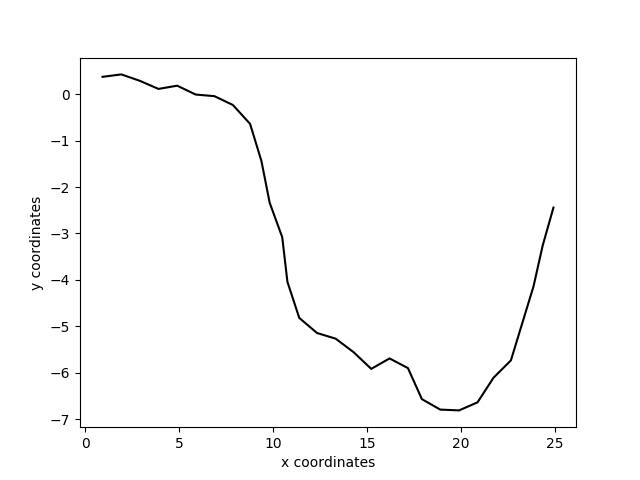
\includegraphics[scale=0.75]{images/relative_example_path.png}
\caption{Relatív random példa útvonal}
\label{fig:relative_path}
\end{figure}

\newpage

\subsection{Python program abszolút elfordulásos esetre}

Itt a generálás módja jóval egyszerűbb, ténylegesen csak egy random szám, amit nem ad hozzá az előző értékhez. Ez esetben az eredmény kevésbé reális, szinte minden útvonalban lesznek olyan szakaszok, ahol jelentős különbség van az előző és az aktuális szög között, így nagyobb törés figyelhető meg a vonalon. A program kimenete a \ref{fig:absolute_path} ábrán látható, valamint ami változott, az a generálási függvény és így a kódrészlet a következő képpen módosult:\\

\begin{python}
def generate_random_angles_absolute(number_of_turns):
    random_angles = []
    for i in range(number_of_turns):
        angle = random.randint(-35, 35)
        random_angles.append(angle)
    return random_angles
    
def calc_path(pos_x, pos_y, steering_angles):
    path = []
    for deg in steering_angles:
        pos_x = pos_x + math.cos(math.radians(deg))
        pos_y = pos_y + math.sin(math.radians(deg))
        path.append((pos_x, pos_y))
    return path
    
rand_angles_absolute = generate_random_angles_absolute(30)

random_absolute_path = calc_path(0, 0, rand_angles_absolute)

x_random_absolute = list(zip(*random_absolute_path))[0]
y_random_absolute = list(zip(*random_absolute_path))[1]

plt.plot(x_random_absolute, y_random_absolute, 'blue')
plt.xlabel("x coordinates")
plt.ylabel("y coordinates")
plt.savefig('absolute_example_path.png')
plt.show()
\end{python}

\begin{figure}[h!]
\centering
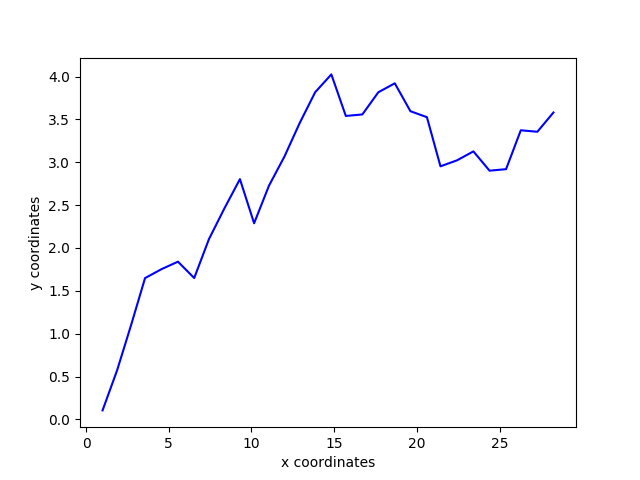
\includegraphics[scale=0.75]{images/absolute_example_path.png}
\caption{Abszolút random példa útvonal}
\label{fig:absolute_path}
\end{figure}

\newpage

\subsection{Ütközés detektálás véletlen útvonalak esetén}
Véletlen útvonalak esetén figyelmbe kell vennünk az esetleges akadályokat. Így a generált utak közül csak az lesz megfelelő, ami ezekbe nem ütközik bele. Tároljuk el ezeket mi magunk a programban, így létrehozva a környezetet. Paraméterek: obstacle(x1, y1, szélesség, magasság). Hozzáadjuk egy listához, hogy később azon végigiterálva meg tudjuk állapítani, hogy melyik obstacle objektumnál történt ütközés.

\begin{python}
obstacle1 = (2, 2, 6, 3)
obstacle2 = (8, 8, 6, 4)
obstacle3 = (15, 2, 4, 2)
obstacle4 = (8, -3, 4, 2)
obstacle5 = (23, -2, 4, 2)

obstacle_list = [obstacle1, obstacle2, obstacle3, obstacle4, obstacle5]
\end{python}

Az előző $ obstacle\_list $ listát végignézve ellenőrizzük, hogy az adott pont az akadály paraméterein belül esik-e. Ha igen, egy hamis változót igazra állítunk, valamint hozzáadjuk az adott pontot egy listához. Itt nem csak az $ x $ és $ y $ koordinátákat adom hozzá, hanem egy $ index $-et is, ami eltárolja, hogy melyik akadály objektumba ütközött az útvonal. Ha hamis, akkor a $ collided $ értéke is hamis marad. Visszatérünk két értékkel:

- volt-e ütközés

- az akadályba ütközött pontok listája

\begin{python}
def is_in_wall(x, y):
    collided = False
    collisions = []
    for index, obstacle in enumerate(obstacle_list):
        if obstacle[0] <= x <= (obstacle[0] + obstacle[2])\
                and obstacle[1] <= y <= (obstacle[1] + obstacle[3]):
            collisions.append((index, x, y))
            collided = True
    return collided, collisions
\end{python}

A már bemutatott $calc\_path$ függvényt kicsit átalakítva végig tudjuk nézni, hogy az útvonalon volt-e ütközés. Itt a for ciklus belsejében az adott pozíciót behelyettesítjük a függvény paraméterlistájába, és az első visszatérési értéket megadva feltételnek, ha az igaz, akkor hozzáadjuk az akadályba ütközött pontokat egy másik listához, amit a második visszatérési érték ad meg. Az útvonal minden eleme ugyanúgy bekerül a $ path $ listába. Majd szintén két értékkel térünk vissza:

- az útvonallal

- az akadályba ütközött pontokkal

\begin{python}
def calc_path(pos_x, pos_y, steering_angles):
    path = []
    collisions = []
    for deg in steering_angles:
        pos_x = pos_x + math.cos(math.radians(deg))
        pos_y = pos_y + math.sin(math.radians(deg))
        if is_in_wall(pos_x, pos_y)[0]:
            collisions.append(is_in_wall(pos_x, pos_y)[1])
        path.append((pos_x, pos_y))
    return path, collisions
\end{python}

Ezt a függvényt az akadályba ütközött pontok normalizálására hívom meg. Rekurzívan eltávolítja a listából a többi listát (bármennyi lehet egymásba ágyazva), így a későbbiekben egyszerűbben hivatkozhatunk a lista tuple típusú elemeire\\
($objektum\_index, x, y$). Az útvonal számító metódust meghívva, a második visszatérési értéke adja meg az ütközött pontokat.

\begin{python}
collision_list = []

def remove_nesting(nested_list):
    for i in nested_list:
        if type(i) == list:
            remove_nesting(i)
        else:
            collision_list.append(i)
            
random_relative_path_collisions = calc_path(0, 0, rand_angles_rel)[1]            
remove_nesting(random_relative_path_collisions)
\end{python}

A listába szervezett akdályokat szemléltetés képpen rajzoljuk ki a területre a \\
$ matplotlib.patches.Rectangle $ funkciót használva. Majd a $ plot() $ függvénnyel az útvonalat kirajzolni, ha pedig volt ütközés, azt legendként jelenítem meg.\\\\
Ismét bemutatnék két példa útvonalat, amelyet a hivatkozott kódrészletek segítségével generáltam ezúttal akadályokkal. Néhány futtatás után kaptunk két hasonló útvonalat, az $ y $ végpontnál talán kissé több az eltérés. Ezt minél több próbálkozással (futtatással) lehetne optimalizálni. \\\\
A \ref{fig:example_nocollision} ábrán az útvonal látható, ahol nem volt ütközés. A \ref{fig:example_collision} ábrán pedig két objektumba is ütközött. Azokat az adatokat látjuk a legendben, ahol történt az ütközés. Az első elem, hogy melyik objektumba, a másik kettő pedig, hogy mely pontokban ütközött $ (x, y) $.

\begin{python}
plt.figure()
rectangle1 = plt.Rectangle((2, 2), 6, 3, fc='blue', ec='red')
plt.gca().add_patch(rectangle1)
rectangle2 = plt.Rectangle((8, 8), 6, 4, fc='blue', ec='red')
plt.gca().add_patch(rectangle2)
rectangle3 = plt.Rectangle((15, 2), 4, 2, fc='blue', ec='red')
plt.gca().add_patch(rectangle3)
rectangle4 = plt.Rectangle((8, -3), 4, 2, fc='blue', ec='red')
plt.gca().add_patch(rectangle4)
rectangle5 = plt.Rectangle((23, -2), 4, 2, fc='blue', ec='red')
plt.gca().add_patch(rectangle5)

plt.plot(x_random_relative, y_random_relative, 'black')
plt.xlabel("x coordinates")
plt.ylabel("y coordinates")
plt.legend(collision_list, loc='upper left', bbox_to_anchor=(0, 1.17),
handletextpad=-0.1, handlelength=0)
plt.savefig('example_nocollision.png')
plt.show()
\end{python}


\begin{figure}[h!]
\centering
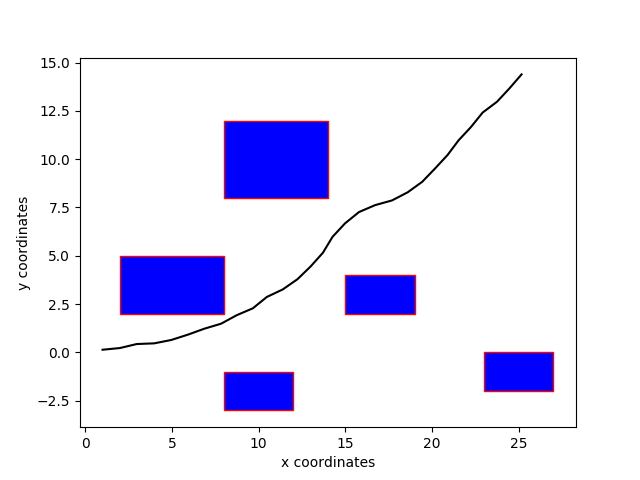
\includegraphics[scale=0.75]{images/example_nocollision.png}
\caption{Példa útvonal ütközés nélkül}
\label{fig:example_nocollision}
\end{figure}



\begin{figure}[h!]
\centering
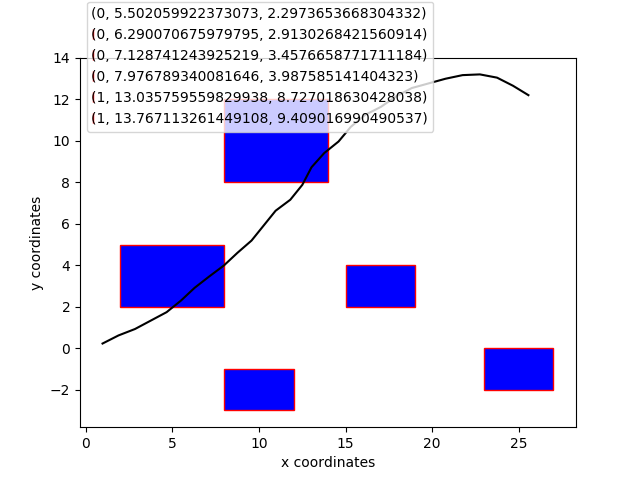
\includegraphics[scale=0.75]{images/example_collision.png}
\caption{Példa útvonal ütközéssel}
\label{fig:example_collision}
\end{figure}

\newpage

\subsection{Végpontok eloszlása, valószínűségi grafikonok}

Ebben az alpontban megvizsgáljuk, hogy különböző paraméterek esetén melyik pozícióba hány alkalommal, illetve milyen valószínűsággel juthatunk el. Legyen az alapértelmezett érték 10 000 mintaszám, tehát ennyi útvonalat fognak a függvények meghatározni. Kigyűjtöm a végpontok $ x $ és $ y $ koordinátáit 2 külön listába, ez alapján ábrázolható az értékek eloszlása.\\\\
Alap esetben legyen az elfordulások száma 30, kanyarodási szög -35$^{\circ}$, +35$^{\circ}$ közötti, generálás módszere relatív, a kezdőpozíció az origó (0, 0).\\\\
Ekkor a \ref{fig:no_obstacles_histogram2d} ábrán a (30, 0) körüli pozíciók a leggyakrabbak, de ugyanúgy gyakori eset például a (-11/+10, 28), melyek 70-70 gyakorisággal fordulnak elő.\\\\
A \ref{fig:obstacles_histogram2d} ábrán csak azokat a végpontokat látjuk, amikor nem volt egyáltalán ütközés. Ez minden esetben, 10 000 generálásnál 7000-7300 közötti rossz útvonalat számol, tehát átlagosan 2850 jó eredményből készül egy ilyen diagram. Az akadályok a \ref{fig:example_collision} vagy a \ref{fig:example_nocollision} ábrákon látható pozíciókban helyezkednek el ebben az esetben. Azt láthatjuk, hogy a leggyakoribb értékek a (12, -24/-26) pontokban lehetnek, szám szerint nagyjából 25-ször fordulnak elő. Tehát az y tengelyt tekintve inkább negatív irányba vinne minket a módszer, persze a pozitív értékeknél is léteznek útvonalak, de már csak 8-10 vagy kevesebb gyakorisággal. A világoskék színnel jelölt négyzetek is átlagban 10-szer, viszonylag gyakran fordulnak elő.



\begin{figure}[h!]
\centering
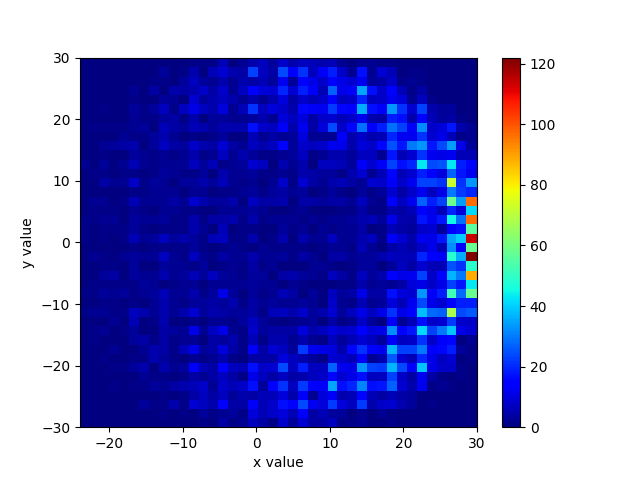
\includegraphics[scale=0.75]{images/no_obstacles_histogram2d.png}
\caption{Elérhető végpontok, ha nincs akadály a pályán}
\label{fig:no_obstacles_histogram2d}
\end{figure}

\begin{figure}[h!]
\centering
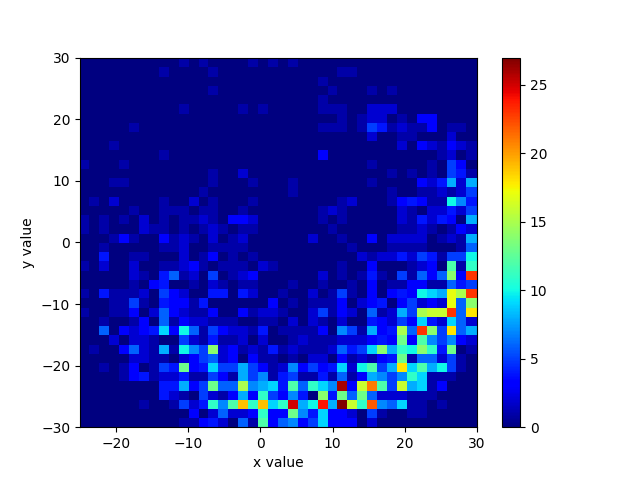
\includegraphics[scale=0.75]{images/obstacles_histogram2d.png}
\caption{Elérhető végpontok, ha vannak akadályok a pályán}
\label{fig:obstacles_histogram2d}
\end{figure}

\newpage

\subsection{Véletlen keresés eredményessége}
Ezen megoldás során inkább a relatív elfordulásos esetet vehetjük életszerűbbnek. Segítségével olyan értékeket kapunk, amelyek a kerék elfordulását határozzák meg az adott lépésben, majd így számolódik a pálya. Mivel ezek random számok, ezért nem lehet szabályozni a végeredményt. A paraméterek megfelelő beállításával kaphatunk az elvárthoz közeli eredményt, ha elegendően sok kimenetet generálunk. Ez viszont még csak egy függvényközelítési probléma, nem tekinthető optimális algoritmusnak a véletlenszerűség miatt. Ugyanakkor a jármű méreteit és irányát sem veszi figyelembe a lépések során.

\Section{Az A* algoritmus megoldása}

Következő lépésben egy olyan megoldást szeretnék bemutatni, amely segítségével bármely pontból eljuthatunk a cél pozícióba, a lehető legkisebb költséggel (jelen esetben a legrövidebb útvonalon).
Az A* algoritmust implementálva az útvonalkereséshez megkaphatjuk az elvárt eredményt. Ez egy olyan kereső eljárás, amelynek alapja a gráfszerű keresés. Minden koordinátát csomópontnak vesz és a kezdőcsúcsból indulva egyesével fűzi hozzá a csúcsokat összekötő éleket mindaddig, míg el nem éri a terminálási feltételt. Ehhez meg kell határozni egy $ f(n) = g(n) + h(n) $ függvényt, ahol $ n $ mindig a következő csúcs az úton, $ g(n) $ a kezdőcsúcstól az n-ig tartó út költsége, és $ h(n) $ egy heurisztikus függvény, amely a két pont közötti legkisebb távolságot veszi fel értékül. Minden lépésben a legkisebb értékkel rendelkező $ f $ értéket választja.
\\

\subsection{A folyamat lépései}

\begin{enumerate}
	\item Egy nyitott listát létrehozunk, majd hozzáadjuk ehhez a kezdőpontot
	\item Ismételjük a következőket, ha a nyitott lista nem üres:
	\begin{enumerate}
		\item Keressük meg a legkisebb $ f $ költségű csomópontot a nyitott listában
		\item Adjuk hozzá a zárt listához
		\item Minden szomszédos csomópontnál:
			\begin{enumerate}
				\item Ha nem járható, vagy ha a zárt listában van, akkor hagyjuk figyelmen kívül, egyébként a következőket csináljuk:
					\begin{enumerate}
						\item Ha nincs a nyitott listában, akkor adjuk hozzá és jelöljük ki a jelenlegi pontot a szülőjének, majd tároljuk el az $ f $, $ g $ és $ h $ költségeit az adott csomópontnak.
						\item Ha már a nyitott listában van, nézzük meg, hogy ez az útvonal jobb-e a $ g $ értéket vizsgálva. Ha ennek az értéke kisebb, akkor ez egy jobb útvonal az előzőnél és meg kell változtatnunk az előző pont szülőjét a jelenlegire és újra kell számítani az $ f $ és $ g $ értékeket.  
					\end{enumerate}
			\end{enumerate}
	\end{enumerate}
	\item Akkor állhatunk meg, ha a cél a zárt listához adódik, így megkaptuk a végső koordinátát, vagy ha nem találta meg valamilyen oknál fogva a célt. 
	\item Végig kell menni céltól a kezdőpontig a pontokon és így kaphatjuk meg az útvonalat
\end{enumerate}

\subsection{A környezet kialakítása}

A célom az volt, hogy egy olyan környezetben tudjam megvalósítani a keresést, amely "végtelen", tehát nincs megadva keret, hogy milyen távolságokba juthatunk el maximum, valamint hogy manuálisan lehessen megadni az akadályok pozícióit és méreteit, ezzel a tesztelést is könnyítve. Ezen kívül maga a környezet lényegében egy Descartes-féle koordináta-rendszer, amelyben a síkban egy $ P $ pont helyzete jól behatárolható $ x $ és $ y $ rendezett számpár alapján. A megjelenítés itt is szintén a matplotlib könyvtár plot() funkciójával fog majd történni.

Létre lehet hozni egy osztályt, amelyet inicializálunk az akadályokkal, ezzel kialakítva a környezetet. Ezeket egy listában tároljuk és ha szeretnénk még hozzáadni akadályokat ugyan úgy az append() funkcióval tehetjük meg. A listának tartalmaznia kell minden koordinátát, ami akadály (tehát a téglalapok keretein belül esőket is). Erre pedig egy másik függvényt hívunk meg, amely for ciklusok segítségével végigiterálva kigyjűt minden pontot az akadályokról. 

\begin{python}
import matplotlib.pyplot as plt
import numpy as np
import math


class AStarPathFinder(object):
    def __init__(self):
        self.obstacles = []
        self.obstacles.append(self.store_obstacle(2, 2, 6, 3))
        self.obstacles.append(self.store_obstacle(8, 8, 6, 4))
        self.obstacles.append(self.store_obstacle(15, 2, 4, 2))
        self.obstacles.append(self.store_obstacle(8, -3, 4, 2))
        self.obstacles.append(self.store_obstacle(23, -2, 4, 2))
        
 	def store_obstacle(self, x1, y1, width, height):
        obstacles = []
        for i in range(x1, (x1 + width + 1)):
            for j in range(y1, (y1 + height + 1)):
                obstacles.append((i, j))
        return obstacles
\end{python}

\subsection{A távolság meghatározása}

A kereső algoritmus alapja, hogy valamilyen módszerrel meg tudjuk határozni a kezdőpont és a végpont közötti távolságot. Ezzel visszakapjuk alapvetően a legrövidebb utat a két pont között. Különböző feltételeket definiálhatunk a mozgással kapcsolatban, így megemlítenék három féle ilyen távolság számítást, amik hatékonyságát a program implementálása során teszteltem.
\begin{itemize}
	\item Manhattan távolság\\
	Egyszerűbb esetekben érdemes alkalmazni, mikor a mozgás csak 4 irányba történhet az adott pontból. \\
	Képlete: 
	\begin{python}
	abs(start[0] - goal[0]) + abs(start[1] - goal[1])
	\end{python}
	\item Diagonális távolság\\
	Akkor érdemes használni, mikor 8 irányban tudunk elmozdulni az adott pontból. Jelen esetben ez is használható lenne, de az elvárt eredményhez ez sem teljesen optimális.\\
	Képlete:
	\begin{python}
	abs(start[0] - goal[0]) + abs(start[1] - goal[1])
	\end{python}
	\item Euklideszi távolság\\
	Ezt a fajta távolság becslést fogom használni, mivel minden irányban el lehet mozdulni és egy reális útvonalat kaphatunk végeredményként.\\
	Képlete a következő függvény visszatérési értéke:
\end{itemize}
\begin{python}
    def calculate_distance(self, start, goal):
        return math.sqrt(((start[0]) - goal[0]) ** 2 +
                         ((start[1]) - goal[1]) ** 2)
\end{python}

A képletek alapján ábrázolt távolságokat a  \ref{fig:distances} képen szemléltetem.

\begin{figure}[h!]
\centering
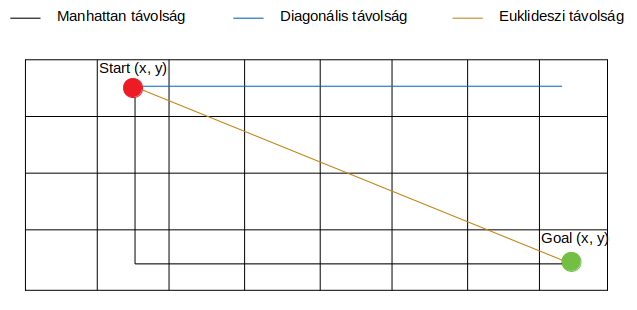
\includegraphics[scale=0.65]{images/distances.png}
\caption{Lehetséges távolságok ábrája a képletek alapján}
\label{fig:distances}
\end{figure}

\subsection{A szomszédos koordináták definiálása}

A megoldás másik elengedhetetlen funkciója, a szomszédos koordináták meghatározása, azok a pontok, amikből az adott lépésben választhatunk. Ez lehetne egyszerűen 4 irány (észak, dél, kelet, nyugat), de esetünkben nem egy labirintus-szerű térképet kell bejárni, hanem egy olyan környezetet, ahol egyedül a lehelyezett akadályokat kell kikerülni, a többi rész pedig szabadon járható. Mivel az algoritmus koordinátánként fogja a lehetőségeket vizsgálni, így az elmozdulás a pontból 8 irányban lehetséges. A \ref{fig:neighbours} ábrán jól látható, hogy az adott koordinátához képest a szomszédokat hogyan kell majd meghatározni a programban.

\begin{figure}[h!]
\centering
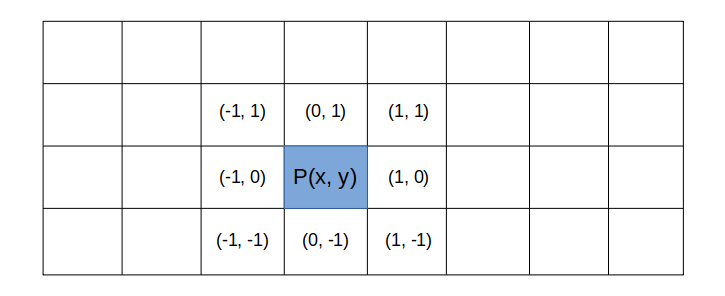
\includegraphics[scale=0.60]{images/neighbours.png}
\caption{Szomszédos koordináták a következő lépés megválasztásához}
\label{fig:neighbours}
\end{figure}

\newpage

Ehhez létre tunuk hozni egy függvényt, ami az aktuális pozíciót megkapja paraméterként. Egy listában eltárolva ezeket a szomszédos pontokat, hozzáadjuk őket egy másik listához, ami az aktuális pozíciót plusz a lehetséges szomszédokat fogja tartalmazni. 

\begin{python}
	def get_neighbours(self, position):
        neighbour = []

        for dx, dy in [(1, 0), (-1, 0), (0, 1), (0, -1),
                       (1, 1), (-1, 1), (1, -1), (-1, -1)]:
            x2 = position[0] + dx
            y2 = position[1] + dy
            neighbour.append((x2, y2))
        return neighbour 
\end{python}

\subsection{A költség meghatározása}

Szükség van egy olyan függvényre is, amely meghatározza a következő pozíció költségét. Ez egyszerűen megoldható, ha minden lépésnek 1 értékű a költsége, viszont ha ez akadályba ütközik, akkor sokkal több. Így biztosan elkerülhető, hogy az algoritmus olyan utat válasszon, ahol akadálynak ütközött.
\begin{python}
    def calc_cost(self, current, next):
        for obstacle in self.obstacles:
            if next in obstacle:
                return 100
        return 1
\end{python}

\subsection{Inputellenőrzés}
Ez a $ check\_points $ metódus csupán azt a célt szolgálja, hogy ellenőrzi a futtatáskor a felhasználó által megadott bemeneti paramétereket (jelen esetben a kezdő- és célpozíció), nem ütköznek-e akadályba. Ha igen, futásidejű hibát dob a program és a többi műveletet nem hajtja végre, ezzel elkerülve a fölösleges erőforrás használatot.
\begin{python}
	def check_points(self, start, end):
        for obstacle in self.obstacles:
            for obs in obstacle:
                if start == obs:
                    raise RuntimeError('Start coordinate is inside 
                    an obstacle!')
                elif end == obs:
                    raise RuntimeError('End coordinate is inside
                    an obstacle!')
\end{python}

\subsection{Implementáció}

Az elején ellenőrizzük, hogy helyesek-e a kezdő és végpont inputok, továbbá deklaráljuk és inicializáljuk a változókat.
\begin{python}
def a_star_search(start, end, map):

    map.check_points(start, end)

    g = {}  
    f = {}  

    g[start] = 0
    f[start] = map.heuristic(start, end)

    closed_nodes = set()
    opened_nodes = {start}
    came_from = {}
\end{python}

\bigskip

Egy while ciklusba kerülnek az ezután következő utasítások. Meg kell választani azt a koordinátát, amelyik a legkisebb $ f $ értékkel rendelkezik a nyitott listában lévőek közül, majd eltárolni jelenlegi pontnak. 
\begin{python}
	while len(opened_nodes) > 0:
        current = None
        current_f_score = None
        for pos in opened_nodes:
            if current is None or f[pos] < current_f_score:
                current_f_score = f[pos]
                current = pos

\end{python}

\bigskip

Ha elértük a végét, végig kell menni az eddig bejárt pontokon visszafelé, hogy megkapjuk a koordináták listáját. Ezeket egyesével hozzáfűzni a $ path $ listához, majd ha ez készen van, a lista elemeit az ellenkező sorrendben kell venni, hogy ne a végéről kezdődjön. Itt kapjuk meg az egész függvény visszatérési értékeit ami az útvonal, és ennek a költsége.
\begin{python}
	if current == end:
            path = [current]
            while current in came_from:
                current = came_from[current]
                path.append(current)
            path.reverse()
            return path, f[end]
\end{python}

\bigskip

A nyitott és zárt lista kezelésére folyamatos eltávolítások és hozzáadások szükségesek:

\begin{python}
	opened_nodes.remove(current)
        closed_nodes.add(current)
\end{python}

\bigskip

A következőkben az algoritmus fő változóinak értékeit fogjuk frissíteni, a szomszédos koordinátákat vizsgálva. Először megnézzük, hogy az adott szomszédos pont már a zárt listában van-e. Ha igen, akkor tovább lépünk, mivel az már fel lett dolgozva. Ha nem, akkor kiszámoltatjuk a költségét és megjelöljük, mint lehetséges következő lépést.\\

Szükséges még megvizsgálni azt is, hogy ha nincs a nyitott listában az adott csomópont. Ilyenkor hozzáadjuk és ha ennek több a költsége, mint az előbb megjelölt lehetséges pontnak, akkor tovább lépünk.\\

Mivel ez olyan ciklusban van, ami az összes szomszédot megvizsgálja, így a végén a legkisebb költségű pontot el lehet tárolni és frissítjük a $ g $, $ h $ és $ f $ változókat.\\

Ha idő előtt kilép a ciklusokból, hibával tér vissza.

\begin{python}
	for neighbour in map.get_neighbours(current):
            if neighbour in closed_nodes:
                continue
            candidate_g = g[current] + map.calc_cost(current, neighbour)

            if neighbour not in opened_nodes:
                opened_nodes.add(neighbour)
            elif candidate_g >= g[neighbour]:
                continue

            came_from[neighbour] = current
            g[neighbour] = candidate_g
            h = map.heuristic(neighbour, end)
            f[neighbour] = g[neighbour] + h

    raise RuntimeError("A* failed to find a solution")
\end{python}

\bigskip

A main függvényben meghívjuk a szükséges metódusokat és kirajzoljuk az eredményt, valamint az akadályokat is szemléltetjük. A képen piros ponttal jelöljük a kezdőpontot, zöld ponttal pedig a végpontot. Az eredményt a \ref{fig:a_star} ábrán láthatjuk.

\begin{python}
if __name__ == "__main__":
    map = AStarPathFinder()

    start = (0, 0)
    goal = (20, 3)

    path, cost = a_star_search(start, goal, map)
    x_coords = list(zip(*path))[0]
    y_coords = list(zip(*path))[1]
    
    plt.figure()
    rectangle1 = plt.Rectangle((2, 2), 6, 3, fc='blue', ec='red')
    plt.gca().add_patch(rectangle1)
    rectangle2 = plt.Rectangle((8, 8), 6, 4, fc='blue', ec='red')
    plt.gca().add_patch(rectangle2)
    rectangle3 = plt.Rectangle((15, 2), 4, 2, fc='blue', ec='red')
    plt.gca().add_patch(rectangle3)
    rectangle4 = plt.Rectangle((8, -3), 4, 2, fc='blue', ec='red')
    plt.gca().add_patch(rectangle4)
    rectangle5 = plt.Rectangle((23, -2), 4, 2, fc='blue', ec='red')
    plt.gca().add_patch(rectangle5)
    
    plt.plot(x_coords, y_coords, 'black')

    plt.plot(start[0], start[1], 'ro')
    plt.plot(goal[0], goal[1], 'go')
    plt.show()
\end{python}


\begin{figure}[h!]
\centering
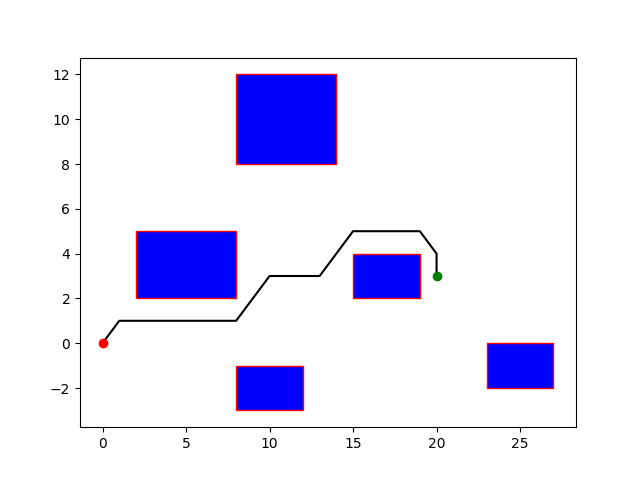
\includegraphics[scale=0.75]{images/a_star.png}
\caption{A* keresés eredménye}
\label{fig:a_star}
\end{figure}

\newpage

\subsection{A* keresés eredményessége}
Ez az algoritmus már útvonal tervezés szempontjából optimálisnak tekinthető. Jóval hatékonyabb a random keresésen alapuló módszernél olyan szempontból, hogy mi határozhatjuk meg a célpozíciót, valamint a fölösleges kanyarodásokat javarészt elkerüli. Az algoritmus a legrövidebb utat adja meg, mindig azt a pontot választja következőnek, amely a legközelebb esik a célhoz (ha az egy járható koordináta). Így ez a megoldás is tehet fölösleges irányváltoztatásokat, mert nem látja az akadályt jóval előre, csak mikor már közel van hozzá. A lehelyezett akadályok elkerülését lényegében ez az implementáció hatékonyan elvégzi, tehát biztos, hogy bármilyen bemenetre jó eredményt fogunk kapni. Másrészt azért is egy hatékony eljárás, mert emlékszik minden olyan pontra, amit már megvizsgált, és ennek függvényében tudja kiválasztani azt, ami a leghamarabb juttatná el a járművet a célba. Az irányt és a jármű méreteit itt sem vesszük figyelembe, így ez is csak egy közelítése az elérni kívánt eredménynek.

\Section{Jármű mozgásának szimulálása}

Az előző két pontban a matematikai számítások alapján készítettem egy szimulációt, ami egy parkolóban ábrázolja a téglatest alakú járművet és be lehet állítani, hogy milyen pozícióból hová jusson el. Szemléltetés képpen készítettem néhány .gif fájlt, amelyek különböző bemenetekre adnak eredményt és szemléltetik a jármű mozgását a fent leírt definíciók alkalmazásával.
\\\\
Lássuk a kódot, kezdve a szükséges importokkal és értéket adunk a konstans változóknak, amik az irányításban és a sebesség megválasztásában játszanak szerepet. Emellett a parkoló kirajzolását végző osztályt példányosítjuk.
\\\\

\begin{python}
import matplotlib.pyplot as plt
import numpy as np
from math import cos, sin, sqrt, atan2, pi
from python.program.navigator import parking_lot

k_distance = 2
k_alpha = 6
k_beta = -2
dt = 0.01

draw = parking_lot.ParkingLot()
\end{python}

\bigskip

Definiáljunk négy tömböt, melynek első két paraméterével lehet a jármű méreteitt állítani, a harmadik pedig mindig 1, hogy az aktuális pozíciót adja vissza (mátrix szorzásnál vehető majd észre). Ez a négy sarkát jelenti a járműnek és az eltolások amiket megadunk, az adott tengely középpontjához mérve értendőek. Az alapértelmezett beállítás 0 radián, ekkor az autó jobbra néz, tehát az $ x $ tengely irányába. A \ref{fig:vehicle_points} ábra szemléltetné ezt a méretezést.

\begin{figure}[h!]
\centering
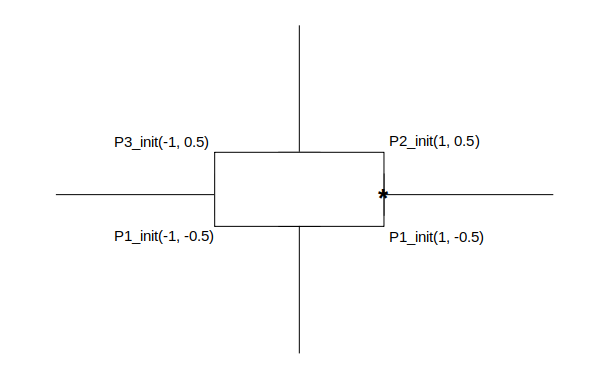
\includegraphics[scale=0.70]{images/vehicle_points.png}
\caption{A jármű négy pontja a programban}
\label{fig:vehicle_points}
\end{figure}

A programban:
\begin{python}
p1_init = np.array([1, -0.5, 1])
p2_init = np.array([1, 0.5, 1])
p3_init = np.array([-1, 0.5, 1])
p4_init = np.array([-1, -0.5, 1])
\end{python}

A rotációs mátrix egy külön függvény lesz, mely mindig az aktuális pozícióra állítja be a járművet.
\begin{python}
def rotation_matrix(x, y, heading_angle):
    return np.array([
        [cos(heading_angle), -sin(heading_angle), x],
        [sin(heading_angle), cos(heading_angle), y],
        [0, 0, 1]
    ])
\end{python}

\bigskip

A következő függvény fogja kirajzolni a járművet és az útvonalat. A pontokat megkapjuk, ha a mátrixokat a numpy.matmul() függvényével összeszorozzuk, valamint a pozíció is mindig az aktuális $ x $ és $ y $ lesz. Következő lépésben a plot() függvény segítségével összekötjük a pontokat egy vonallal, így lesz látható végig a jármű. Valamint még egy csillagot helyeztem az első részére, hogy tudjuk merre van a jármű eleje. Itt rajzoljuk ki a parkolót is, valamint kék szaggatott vonallal az útvonalat, amit egy másik függvény számol. A .gif animációhoz a képeket pedig a savefig() függvénnyel mentem le, mindig az adott lépésszámot kapja a kép neve, hogy ne íródjanak felül és legyen egy sorrend a mozgókép készítéshez.

\begin{python}
def plot_vehicle(x, y, heading_angle, x_path, y_path, steps):
    """
    Plotting the vehicle and it's path using the rotation matrix
    for visualizing.
    Plotting the parking lot as well.
    :param x: actual x position of the vehicle
    :param y: actual y position of the vehicle
    :param heading_angle: heading angle
    :param x_path: x trajectory
    :param y_path: y trajectory
    :param steps: number of steps in the motion, using for generating
    images with numbered names
    :return: none
    """
    r = rotation_matrix(x, y, heading_angle)

    p1 = np.matmul(r, p1_init)
    p2 = np.matmul(r, p2_init)
    p3 = np.matmul(r, p3_init)
    p4 = np.matmul(r, p4_init)

    plt.plot([(p1[0] + p2[0]) / 2], p1[1], 'k*')

    plt.plot([p1[0], p2[0]], [p1[1], p2[1]], 'k-')
    plt.plot([p2[0], p3[0]], [p2[1], p3[1]], 'k-')
    plt.plot([p3[0], p4[0]], [p3[1], p4[1]], 'k-')
    plt.plot([p4[0], p1[0]], [p4[1], p1[1]], 'k-')

    draw.plot_parking_lot()

    plt.plot(x_path, y_path, 'b--')
    plt.savefig('pictures/'f'fig-0{steps}.png')

\end{python}

\bigskip

A következő metódus fogja a jármű mozgatását, irányba állítását végezni a háttérben. Megadja magát az útvonalat, amit be kell járni. A szükséges változók értéket kapnak. A $ distance $ azért szerepel kétszer, mert az folyamatosan csökkenni fog, ahogy haladunk a cél felé, viszont szükség lesz a kezdőértékére is, hogy hatékonyabban tudjuk kontrollálni a sebességet ezáltal. Természetesen, ahogy az A* algoritmusnál, úgy itt is az Euklideszi távolsággal való számítás fog optimális eredményt adni.

\begin{python}
def moving_vehicle(x_start, y_start, start_heading_angle, x_goal,
 y_goal, goal_heading_angle):
    """
    Calculates the trajectory and calls vehicle plotting
    function to visualize it
    :param x_start: x start coordinate of vehicle
    :param y_start: y start coordinate of vehicle
    :param start_heading_angle: vehicle's heading angle at the start
    :param x_goal: x goal coordinate of vehicle
    :param y_goal: y goal coordinate of vehicle
    :param goal_heading_angle: vehicle's target heading angle
    at the goal position
    :return: none
    """
    x = x_start
    y = y_start
    heading_angle = start_heading_angle

    x_diff = x_goal - x
    y_diff = y_goal - y
    distance_init = sqrt(x_diff**2 + y_diff**2)
    distance = sqrt(x_diff**2 + y_diff**2)

    x_path = []
    y_path = []
\end{python}

\bigskip

A következőkben a távolság újraszámolódik, ugyanis ez minden lépésnél változni fog. A ciklus addig tart, amíg a céltól való távolság el nem ér egy nagyon kicsi értéket, jelen esetben a 0.01-et. Ezen kívül itt hozom létre azokat a szögeket, amik a \ref{fig:moving_vehicle} ábrán láthatóak. Tehát $ alpha $ az a szög, ami a jármű jelenlegi pozícióját mutató vektor és a cél felé mutató vektor által bezárt szög. Ugyanakkor a $ beta $ szög a célba érkezéshez megadott szög és a jelenlegi irány közötti szög lenne. Ezen felül a sebességet $ v $ változóként definiálom a távolsággal arányosan, valamint egy $ steering $ változót, ami végzi majd a jármű forgatását, tehát a kanyarodási szög, ami a \ref{fig:moving_vehicle} ábrán $ \gamma $ jelzéssel szerepel.

\begin{python}
while distance > 0.01:
        x_diff = x_goal - x
        y_diff = y_goal - y

        distance = sqrt(x_diff**2 + y_diff**2)
        alpha = atan2(y_diff, x_diff) - heading_angle
        beta = goal_heading_angle - heading_angle - alpha

        v = k_distance*distance
        steering = k_alpha*alpha + k_beta*beta
\end{python}

\bigskip

A sebesség kontrollálása következik. Színvonalasabb az animáció, ha a sebességet az első néhány méteren csökkentjük, vagyis utána fog növekedni a távolság függvényében. Ezzel a lassabb elindulást tehetjük láthatóvá, majd a gyorsítást. A célhoz közel pedig szintén lelassul, ez is a távolságtól függ. Másrészt beállítjuk, hogy tolasson a jármű, ha az $ alpha $ szög nagyobb mint $ \dfrac{\pi}{2} $ vagy kisebb, mint $ -\dfrac{\pi}{2} $ ( $ \alpha $ > 90$^{\circ}$ vagy $ \alpha $ < - 90$^{\circ}$ ). Ezzel a parkolóból hátrafelé kiállást valósíthatjuk meg. A tolatás sebessége egy állandó érték, ezzel megakadályozva, hogy túl gyorsan tolasson ki a távolságbecslés miatt.

\begin{python}
        if distance > distance_init - 1:
            v = v/3
        elif distance > distance_init - 2:
            v = v/2

        if alpha > pi/3 or alpha < -pi/3:
            v = -9
\end{python}

\bigskip

A $ \delta $ szöget itt a $ heading\_angle $ jelöli, ami a kanyarodás függvényében változik. Az $ x $ és $ y $ pozíciókat  hozzáadom az útvonl tárolásához létrehozott tömbökhöz, majd a kirajzoláshoz megjelenítek két nyilat, melyek a kezdő és végpozíciót reprezentálják. Ez után a már bemutatott $ plot\_vehicle $ metódus segítségével kirajzolom az útvonalat és a járművet. Ha ez a $ while $ cikluson belül történik, akkor minden lépésről képet generál, és ezekből készítettem különböző esetekre .gif animációkat. Mivel linux környezetben dolgozom, ezeket a képeket egy terminálból lefuttatott paranccsal át tudtam konvertálni: convert -delay 2 -loop 0 \$(ls -1 *.png | sort -V) animation.gif

\begin{python}
 	heading_angle = heading_angle + steering*dt

        x = x + v*cos(heading_angle)*dt
        y = y + v*sin(heading_angle)*dt
        x_path.append(x)
        y_path.append(y)

        plt.cla()
        plt.arrow(x_start, y_start, cos(start_heading_angle),
                  sin(start_heading_angle), color='r', width=0.1)
        plt.arrow(x_goal, y_goal, cos(goal_heading_angle),
                  sin(goal_heading_angle), color='g', width=0.1)
        plot_vehicle(x, y, heading_angle, x_path, y_path, len(x_path))
\end{python}

A $ main $ függvényben megadjuk a szükséges paramétereket és meghívjuk a \\ $ moving\_vehicle $ metódust. Az így kapott eredményeket a dolgozatom "animations" nevű mappájában megtalálható.

\begin{python}
if __name__ == '__main__':
    x_start = 6.5
    y_start = 8
    start_heading_angle = pi/2
    x_goal = 18.5
    y_goal = 9
    goal_heading_angle = -pi/2

    print("Start x: %.2f m\nStart y: %.2f m\nStart heading angle:
     %.2f rad\n" % (x_start, y_start, start_heading_angle))
    print("Start x: %.2f m\nGoal y: %.2f m\nGoal heading angle:
     %.2f rad\n" % (x_goal, y_goal, goal_heading_angle))
    moving_vehicle(x_start, y_start, start_heading_angle, x_goal,
     y_goal, goal_heading_angle)
\end{python}

\subsection{A jármű mozgatásának eredményessége}
Ez a megoldás jobban eltér az előzőektől. Itt az volt a szempont, hogy belekalkulálva a jármű mozgásához kapcsolódó irányváltoztatásokat és többek között a sebességet egy olyan ívelt pályán tudjunk eljutni a célba, ami az adott feltételek mellett reálisnak vehető. Tehát a sebességet, valamint a mozgás ívét is konstans értékekkel változtatva különböző eredményeket kaphatunk, mint útvonal. Ezzel a logikával könnyedén tudunk szimulációkat készíteni, mivel magát a járművet is megjeleníti, mint egy téglalap alakú objektum. Az eredmény képeket .gif formátumba átkonvertálva pedig animációkat készíthetünk. Összességében egy üres parkolóban történő navigálásra használható ez a fajta heurisztika. Amit még itt szerettem volna megvalósítani az egy nem üres parkolós környezet. Eredményesebb lenne, ha be tudná azonosítani más járművek pozícióját és észlelni, valamint elkerülni az ütközést ezen objektumokkal. 
